% Original source-bound construction visual, 6 November 2026.
\begin{figure}[p]
\centering
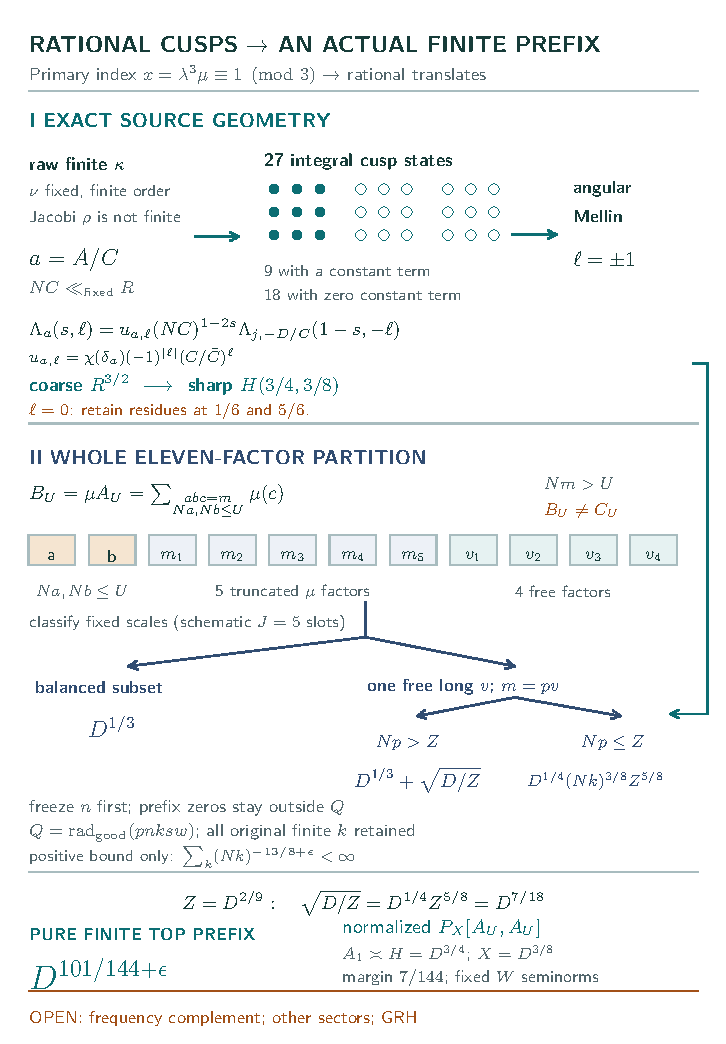
\includegraphics[width=350pt]{figures/ramified-cusp-prefix.pdf}
\caption{The rational-cusp construction feeds a whole-factor partition of the
original coefficient. Here $R=N\mathfrak t$, the angular orders are
$\ell=\pm1$, and the pure finite-prefix budget uses $D\ge2^{64}$,
fixed character data and the displayed profile seminorms.
The positive $\mathfrak k$ majorant requires sufficiently small
$\epsilon<5/8$; the actual cutoff remains finite.
The diagram shows a proof construction, not measured energy.
The full signed kernel and GRH remain open.}
\label{rg:workflow}
\end{figure}
